\section*{Random Matrix Preliminaries}

Let $X\in\R^{n\times N}$ have independent rows $x_t^\top\sim\N(0,\Sigma)$, $t=1,\ldots,n$, so that $W=X^\top X$ has the Wishart law $\mathcal W_N(n,\Sigma)$ and $S=W/n$ is the sample covariance matrix with known zero mean. When the mean is estimated, all statements hold with $n$ replaced by $n-1$, since the centred cross-product matrix is $\mathcal W_N(n-1,\Sigma)$ \citep[Ch.~3]{muirhead1982aspects}. The aspect ratio is $q=N/n$. Throughout, $\lambda_1\geq\cdots\geq\lambda_N$ denote the eigenvalues of $S$ and $\mu_S=N^{-1}\sum_i\delta_{\lambda_i}$ its empirical spectral measure. This section collects the tools of random matrix theory used later. Its purpose is to fix conventions and to give self-contained derivations of the few facts on which the new results rest. Comprehensive treatments are \citet{bai2010spectral}, \citet{anderson2010introduction}, \citet{tao2012topics}, \citet{erdos2017dynamical} and, with an eye to applications in finance, \citet{bouchaud2011financial}, \citet{bun2017cleaning} and \citet{potters2020first}.

\subsection*{Resolvents, Stieltjes transforms and the Marchenko--Pastur law}

For $z\in\C\setminus\R$ the resolvent is $G_S(z)=(z-S)^{-1}$ and the Stieltjes transform of $\mu_S$ is
\[
 g_S(z)=\frac1N\tr G_S(z)=\int\frac{\mu_S(\dd x)}{z-x}.
\]
The function $g_S$ is analytic off the spectrum, maps the upper half-plane to the lower half-plane, and behaves like $1/z$ at infinity, with the Laurent expansion $g_S(z)=\sum_{k\geq0}m_k z^{-k-1}$ in terms of the moments $m_k=N^{-1}\tr S^k$. A probability density is recovered from its Stieltjes transform through the inversion formula $\rho(x)=\pi^{-1}\lim_{\eta\downarrow0}\Imag g(x-i\eta)$. Convergence of Stieltjes transforms at every $z\in\C\setminus\R$ is equivalent to weak convergence of the underlying measures. The entire asymptotic theory of spectra can therefore be phrased in terms of $g$.

The self-consistent equation for $g_S$ follows from a leave-one-out argument that I record because the same algebra reappears in the outlier and cleaning formulas. Write $S=n^{-1}\sum_t x_tx_t^\top$ and $S_{(t)}=S-n^{-1}x_tx_t^\top$, with resolvent $G_{(t)}=(z-S_{(t)})^{-1}$. Taking the trace of the identity $zG_S-SG_S=I$ gives $zNg_S-n^{-1}\sum_t x_t^\top G_Sx_t=N$. The Sherman--Morrison formula gives $G_S=G_{(t)}+G_{(t)}x_tx_t^\top G_{(t)}/(n-x_t^\top G_{(t)}x_t)$, whence
\[
 \frac1n x_t^\top G_Sx_t=\frac{n^{-1}x_t^\top G_{(t)}x_t}{1-n^{-1}x_t^\top G_{(t)}x_t}.
\]
Because $x_t$ is independent of $G_{(t)}$, the quadratic form $n^{-1}x_t^\top G_{(t)}x_t$ concentrates around $n^{-1}\tr(\Sigma G_{(t)})$, and $G_{(t)}$ differs from $G_S$ by a rank-one perturbation whose normalised trace is $O(N^{-1})$. When $\Sigma=I$ the quadratic form is therefore $qg_S+o(1)$, and dividing the trace identity by $N$ yields $zg-g/(1-qg)=1$. In polynomial form,
\begin{equation}
 qz\,g(z)^2-(z-1+q)\,g(z)+1=0.
 \label{eq:mp-quadratic}
\end{equation}
The root with $g(z)\sim1/z$ at infinity is $g(z)=[z-1+q-\sqrt{(z-1+q)^2-4qz}\,]/(2qz)$. The discriminant vanishes at $\lambda_\pm=(1\pm\sqrt q)^2$, and the inversion formula yields the Marchenko--Pastur density
\begin{equation}
 \rho_q(x)=\frac{\sqrt{(\lambda_+-x)(x-\lambda_-)}}{2\pi qx},\qquad x\in[\lambda_-,\lambda_+],
 \label{eq:mp-density}
\end{equation}
together with an atom of mass $1-1/q$ at the origin when $q>1$ \citep{marchenko1967distribution}. The edges are also the almost sure limits of the extreme eigenvalues \citep{geman1980limit,bai1993limit}. Figure~\ref{fig:mp-family} shows the family. As $q$ grows the bulk spreads from a point mass at one to an interval that touches the origin at $q=1$. This spreading is the mechanism behind every cost of dimensionality discussed in this paper.

\begin{figure}[htbp]
\centering
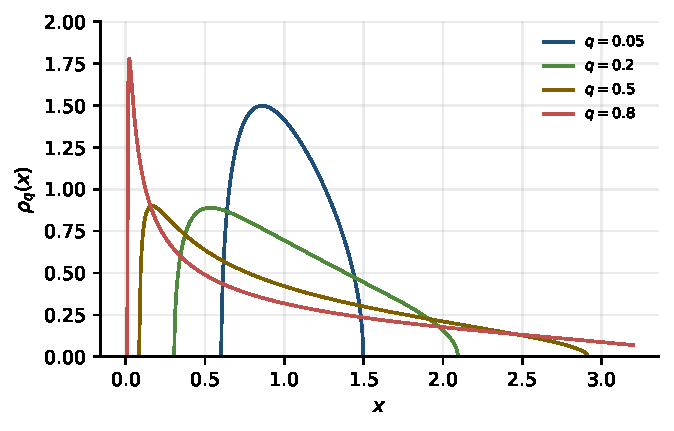
\includegraphics[width=0.62\textwidth]{figures/mp_family.pdf}
\caption{Marchenko--Pastur densities $\rho_q$ for four aspect ratios. The edges $(1\pm\sqrt q)^2$ are the zeros of the discriminant of the quadratic \eqref{eq:mp-quadratic}. The left edge reaches the origin at $q=1$, where $\log\det S$ diverges.}
\label{fig:mp-family}
\end{figure}

The moments of $\rho_q$ follow from \eqref{eq:mp-quadratic} without integration. Writing $h(x)=\sum_k m_kx^k=z\,g(z)$ with $x=1/z$, the quadratic becomes $h=1+xh(1-q+qh)$, which is equivalent to the recursion
\begin{equation}
 m_k=(1-q)\,m_{k-1}+q\sum_{j=0}^{k-1}m_j\,m_{k-1-j},\qquad m_0=1.
 \label{eq:mp-recursion}
\end{equation}
Its solution is the Narayana polynomial $m_k=\sum_{j=0}^{k-1}\tfrac1k\binom kj\binom k{j+1}q^j$, whose coefficients count non-crossing partitions of $\{1,\ldots,k\}$ by number of blocks \citep{stanley1999enumerative,nica2006lectures}. The first four are $1$, $1+q$, $1+3q+q^2$ and $1+6q+6q^2+q^3$. At $q=1$ the Narayana numbers sum to the Catalan numbers, which are also the even moments of the semicircle law $\rho_{\rm sc}(x)=(2\pi)^{-1}\sqrt{4-x^2}$ of \citet{wigner1955characteristic,wigner1958distribution}. The Lean file accompanying this paper verifies with exact integer arithmetic that the recursion \eqref{eq:mp-recursion} generates the Narayana polynomials up to order ten, that the semicircle recursion generates the Catalan numbers up to order twelve, and that the Narayana rows sum to the Catalan numbers. At finite $n$ the exact Wishart moments differ from the limits by explicit corrections. Using $\E W^2=n(n+N+1)I$ and $\E\tr W^3=nN(n^2+N^2+3nN+3n+3N+4)$ for $\Sigma=I$ \citep{muirhead1982aspects},
\[
 \frac1N\E\tr S^2=1+q+\frac1n,\qquad
 \frac1N\E\tr S^3=1+3q+q^2+\frac{3(1+q)}n+\frac4{n^2}.
\]
Both formulas are checked by simulation in the numerical section.

For general $\Sigma$ with limiting spectral distribution $H$ the same leave-one-out argument, now keeping track of $n^{-1}\tr(\Sigma G_{(t)})$, gives the Marchenko--Pastur--Silverstein equation
\begin{equation}
 g(z)=\int\frac{H(\dd\tau)}{z-\tau\,w(z)},\qquad w(z)=1-q+qz\,g(z),
 \label{eq:silverstein}
\end{equation}
\citep{silverstein1995empirical}. The function $w$ is a subordination function: the sample resolvent evaluated at $z$ behaves on average like the population resolvent evaluated at $z/w(z)$, rescaled. Three facts used below are direct consequences of \eqref{eq:silverstein}. First, for $H=\delta_1$ it reduces to $g=1/(z-w)$, which is \eqref{eq:mp-quadratic}. Second, a population eigenvalue $\ell$ outside the bulk produces a sample outlier at the solution $z$ of $z=\ell\,w(z)$, the value at which the integrand of \eqref{eq:silverstein} becomes singular. Third, the expected projection of a sample eigenvector on the population eigenbasis is a function of $w$ evaluated at the sample eigenvalue. That fact is the basis of the oracle nonlinear shrinkage formula
\begin{equation}
 \xi(\lambda)=\frac{\lambda}{|1-q+q\lambda\,g(\lambda-i0)|^2}=\frac{\lambda}{|w(\lambda-i0)|^2}
 \label{eq:rie}
\end{equation}
of \citet{ledoit2011eigenvectors} and the rotationally invariant estimator of \citet{bun2016rotational}. In this estimator, each sample eigenvalue is replaced by $\xi(\lambda_i)$, with $g$ evaluated from the sample spectrum at a small distance $\eta$ below the real axis.

\subsection*{Free probability}

The Silverstein equation is an instance of free multiplicative convolution. For a probability measure $\mu$ on $[0,\infty)$ with moment generating function $\psi_\mu(z)=\sum_{k\geq1}m_kz^k$, let $\chi_\mu$ be the inverse of $\psi_\mu$ near the origin and define the $S$-transform $S_\mu(w)=\chi_\mu(w)(1+w)/w$. \citet{voiculescu1991limit} showed that large rotationally invariant matrices behave as free random variables, and that the spectrum of a product of free positive elements has $S$-transform equal to the product of the $S$-transforms \citep{voiculescu1992free,mingo2017free}. From \eqref{eq:mp-recursion}, $\psi=h-1$ satisfies $\psi=x(1+\psi)(1+q\psi)$, so $\chi(w)=w/[(1+w)(1+qw)]$ and
\[
 S_{\rm MP}(w)=\frac1{1+qw}.
\]
The spectrum of $S=\Sigma^{1/2}S_0\Sigma^{1/2}$, with $S_0$ white Wishart, is then the free multiplicative convolution $H\boxtimes\rho_q$, whose $S$-transform is $S_H(w)/(1+qw)$. Two consequences are worth stating. Because $S_{\rm MP}$ is a M\"obius map, cleaning a sample spectrum amounts to a free deconvolution, which is what \eqref{eq:rie} implements eigenvalue by eigenvalue. Free cumulants of $\rho_q$ are all equal to $q^{k-1}$, which is the free-probability statement of the Narayana formula. The additive analogue is the $R$-transform, $R_\mu=g_\mu^{-1}(w)-1/w$. The semicircle has $R(w)=\sigma^2w$, which drives the dynamics studied later.

\subsection*{Canonical correlations and the Jacobi ensemble}

Partition $x_t=(x_{t,1}^\top,x_{t,2}^\top)^\top$ with blocks of dimensions $p\leq r$, and partition $S$ conformably. The squared sample canonical correlations $\hat\rho_1^2\geq\cdots\geq\hat\rho_p^2$ are the eigenvalues of $S_{11}^{-1}S_{12}S_{22}^{-1}S_{21}$. Equivalently, if $P_1$ and $P_2$ are the orthogonal projections of $\R^n$ onto the column spaces of the two data blocks, they are the nonzero eigenvalues of $P_1P_2P_1$. When the blocks are independent, the column spaces are uniformly distributed and independent. The $\hat\rho_k^2$ then form a Jacobi (MANOVA) ensemble, with joint density proportional to $\prod_k x_k^{(r-p-1)/2}(1-x_k)^{(n-r-p-1)/2}\prod_{j<k}|x_j-x_k|$ on $[0,1]^p$ \citep{muirhead1982aspects,johnstone2008multivariate}. In free-probability terms, $P_1$ and $P_2$ are asymptotically free projections of traces $c_1=p/n$ and $c_2=r/n$, and the limiting law of $P_1P_2P_1$ is the free multiplicative convolution of two Bernoulli laws \citep{collins2005product}. Its absolutely continuous part, for $c_1\le c_2$ and $c_1+c_2<1$, is the law of \citet{wachter1980limiting},
\begin{equation}
 w_{c_1,c_2}(x)=\frac{\sqrt{(x-\omega_-)(\omega_+-x)}}{2\pi c_1\,x(1-x)},\qquad
 \omega_\pm=\Bigl(\sqrt{c_1(1-c_2)}\pm\sqrt{c_2(1-c_1)}\Bigr)^2.
 \label{eq:wachter}
\end{equation}
This density has unit mass on $[\omega_-,\omega_+]$ and mean $c_2$. Figure~\ref{fig:wachter} compares it with simulated canonical correlations of independent Gaussian blocks. The upper edge satisfies $\omega_+<1$ exactly when $c_1+c_2<1$, which keeps $\log(1-x)$ bounded on the support. That boundedness drives the information laws below.

\begin{figure}[htbp]
\centering
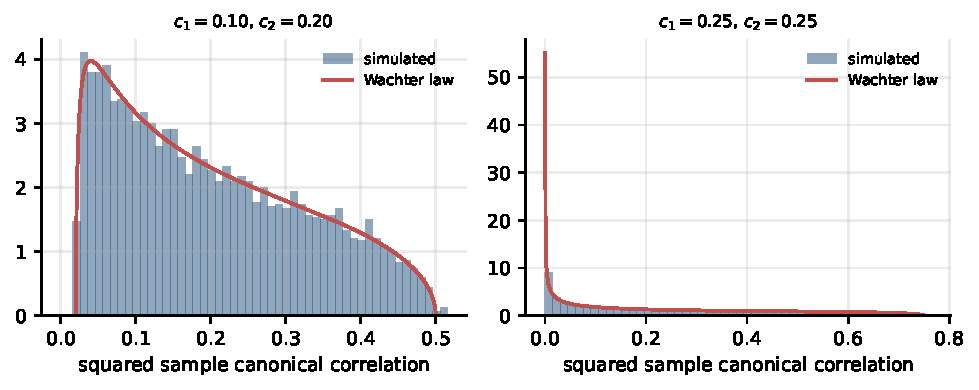
\includegraphics[width=\textwidth]{figures/wachter.pdf}
\caption{Squared sample canonical correlations of independent Gaussian blocks (30 replications) and the Wachter law \eqref{eq:wachter}. Left: $n=1000$, $p=100$, $r=200$. Right: $n=600$, $p=r=150$. The upper edge $\omega_+$ stays below one because $c_1+c_2<1$.}
\label{fig:wachter}
\end{figure}

\subsection*{Spiked models and phase transitions}

Real covariance matrices are not white, and the structures that matter in finance are low-rank: a market factor, a handful of sectors, a few dependence directions between blocks. The spiked covariance model $\Sigma=I+\sum_{k\leq K}(\ell_k-1)v_kv_k^\top$ with fixed $K$ captures this. Substituting $H=(1-K/N)\delta_1+N^{-1}\sum_k\delta_{\ell_k}$ into \eqref{eq:silverstein} and using the outlier condition $z=\ell w(z)$ with the Marchenko--Pastur subordination function gives the explicit relation
\begin{equation}
 \lambda(\ell)=\ell\Bigl(1+\frac q{\ell-1}\Bigr),\qquad\ell>1+\sqrt q.
 \label{eq:bbp}
\end{equation}
The derivation is short. With $w=z/\ell$, the bulk relation $(w-1+q)(z-w)=qz$ becomes $(z/\ell-1+q)(1-1/\ell)=q$, which rearranges to \eqref{eq:bbp}. The solution leaves the bulk only when $\lambda(\ell)>\lambda_+$. Since $\lambda(1+\sqrt q)=(1+\sqrt q)^2$, the threshold is $\ell_c=1+\sqrt q$, the Baik--Ben Arous--P\'ech\'e (BBP) transition \citep{baik2005phase,baik2006eigenvalues}. Above the threshold the sample eigenvector $u_k$ makes a nontrivial angle with $v_k$,
\begin{equation}
 \langle u_k,v_k\rangle^2\to\frac{1-q/(\ell_k-1)^2}{1+q/(\ell_k-1)}.
 \label{eq:overlap}
\end{equation}
Below it, the overlap vanishes \citep{paul2007asymptotics,benaych2011eigenvalues,bloemendal2016principal}. Inverting \eqref{eq:bbp} gives the quadratic $\ell^2-(\lambda+1-q)\ell+\lambda=0$, whose larger root is the population spike implied by an observed outlier $\lambda$, and \eqref{eq:overlap} then predicts how reliable the corresponding eigenvector is. The Lean file certifies the threshold identity, the vanishing of the overlap numerator at the threshold and the inversion quadratic. Fluctuations of the largest eigenvalue at the edge follow the Tracy--Widom laws \citep{tracy1994level,tracy1996orthogonal,johnstone2001distribution}. They are not needed here.

The analogous transition for canonical correlations is less familiar and plays a central role in the information frontier below. Suppose the blocks have a single nonzero population canonical correlation $t$. The theory of \citet{bao2019canonical} shows that the leading sample canonical correlation separates from the Wachter bulk if and only if $t>t_c$, and otherwise sticks to $\omega_+$. In the parametrisation I use, which simulation confirms in the numerical section, the threshold and the separated limit are
\begin{equation}
 t_c^4=\frac{c_1c_2}{(1-c_1)(1-c_2)},\qquad
 \hat\rho_1^2\to\gamma(t)=t^2\Bigl(1-c_1+\frac{c_1}{t^2}\Bigr)\Bigl(1-c_2+\frac{c_2}{t^2}\Bigr)\quad(t>t_c).
 \label{eq:cca-spike}
\end{equation}
At $t=t_c$, $\gamma(t_c)=c_1(1-c_2)+c_2(1-c_1)+2t_c^2(1-c_1)(1-c_2)=\omega_+$, because $t_c^2(1-c_1)(1-c_2)=\sqrt{c_1c_2(1-c_1)(1-c_2)}$. At $t=1$, $\gamma=1$. The Lean file proves the threshold identity under the defining constraint on $t_c$. As with \eqref{eq:bbp}, the map $t\mapsto\gamma(t)$ is invertible above the threshold. A quadratic in $t^2$ recovers a debiased canonical correlation from an observed outlier.

\subsection*{Logarithmic spectral statistics}

The functionals at the heart of this paper are logarithmic. The Bartlett decomposition writes $W=LL^\top$ for $\Sigma=I$, with $L$ lower triangular, independent entries, $L_{ii}^2\sim\chi^2_{n-i+1}$ and $L_{ij}\sim\N(0,1)$ for $i>j$ \citep[Ch.~3]{muirhead1982aspects}. Hence $\log\det W=\sum_{i=1}^N\log L_{ii}^2$ is a sum of independent log-chi-square variables. Since $\E\log\chi^2_k=\psi(k/2)+\log2$ and $\Var\log\chi^2_k=\psi'(k/2)$, with $\psi$ the digamma function, and since $\det S=\det\Sigma\,\det(W_0/n)$ for a white Wishart $W_0$, one obtains for every $\Sigma$ the exact identities
\begin{equation}
 \begin{gathered}
 \ell_n(N)\equiv\E\log\det S-\log\det\Sigma=\sum_{i=1}^N\Bigl[\psi\Bigl(\frac{n-i+1}2\Bigr)-\log\frac n2\Bigr],\\
 \Var\log\det S=\sum_{i=1}^N\psi'\Bigl(\frac{n-i+1}2\Bigr).
 \end{gathered}
 \label{eq:logdet}
\end{equation}
Using $\psi(x)=\log x-1/(2x)+O(x^{-2})$ and $\psi'(x)=1/x+O(x^{-2})$, a Riemann-sum argument gives
\begin{equation}
 \frac1N\ell_n(N)\to\varphi(q)\equiv\int\log x\,\rho_q(\dd x)=-1-\frac{1-q}q\log(1-q),\qquad
 \Var\log\det S\to-2\log(1-q),
 \label{eq:phi}
\end{equation}
because $N^{-1}\sum_{i\le N}\log(1-(i-1)/n)\to q^{-1}\int_0^q\log(1-u)\,\dd u$. The second-order term is explicit as well. An Euler--Maclaurin expansion shows $\ell_n(N)=N\varphi(N/n)+\tfrac12\log(1-N/n)+o(1)$, which is the mean correction in the central limit theorem for linear spectral statistics of \citet{bai2004clt}, with variance $-2\log(1-q)$ in the real case. Thus the log-determinant is biased downward by an amount proportional to $N$, while its fluctuations remain of order one. The bias is the Jensen gap of the logarithm integrated against the spreading of the Marchenko--Pastur bulk, and it is the seed of every information law in the next section. The exact formula \eqref{eq:logdet} and its limit underlie the high-dimensional entropy estimators of \citet{ahmed1989entropy}, \citet{misra2005estimation} and \citet{cai2015law}, and the corrected likelihood-ratio tests of \citet{bai2009corrections} and \citet{jiang2013central}.
